\subsection{Function-Space Compactness}

% **Role:** convergence of functions and analytic approximation.
%
% Equicontinuity, Arzela--Ascoli, compactness in function spaces, Banach-space preview.


Function-space compactness treats functions as points. Supremum metrics preview Banach spaces, Baire category describes generic behavior, and equicontinuity leads to Arzela--Ascoli.

\begin{theorem} \label{thm:complete-supremum-metric-space} \hlt{Completeness of the Supremum Metric}\\
The metric space $C_b(X)$ with metric $d(f,g)=\norm{f-g}_{\infty}$ is complete.
\begin{proof}
Let $(f_n)$ be Cauchy in $C_b(X)$. Then Theorem \ref{thm:uniform-cauchy-criterion} gives a function $f$ with $f_n\rightrightarrows f$. By Theorem \ref{thm:uniform-convergence-preserves-continuity}, $f$ is continuous. For some $n$, $\norm{f-f_n}_{\infty}<1$, hence $f_n$ is bounded, thus $f\in C_b(X)$ and $\norm{f_n-f}_{\infty}\to0$.\\
\hlt{Structural Commentary}: Uniform Cauchy convergence builds the limit inside the same function space.\\
\hlt{Key Insight}: Completeness of $\C$ plus uniform convergence makes $C_b(X)$ complete.
\end{proof}
\end{theorem}

\begin{definition} \label{def:bounded-target-metric-function-space} \hlt{Bounded Target Metric for All Functions}\\
For metric spaces $(X,d_X)$ and $(Y,d_Y)$, let $\mathcal{F}=Y^X$ and set $\rho(y,z)\defeq\frac{d_Y(y,z)}{1+d_Y(y,z)}$ and $d_\rho(f,g)\defeq\sup_{x\in X}\rho(f(x),g(x))$.\\
Then $\rho<1$, so $d_\rho$ is finite on all of $\mathcal{F}$; $d_\rho$-convergence is uniform convergence measured by $d_Y$.
\end{definition}

\begin{theorem} \label{thm:bounded-target-metric-function-space-completeness} \hlt{Completeness and Closed Subspaces for $d_\rho$}\\
If the target metric space $(Y,d_Y)$ is complete, then:
\begin{enumerate}[label=(\roman*)]
\setlength{\itemsep}{0pt}
\item $(\mathcal{F},d_\rho)$ is complete;
\item $\mathcal{F}_b\defeq\{f\in\mathcal{F}:f(X)\text{ is }d_Y\text{-bounded}\}$ is closed in $\mathcal{F}$;
\item $C(X,Y)$ is closed in $\mathcal{F}$.
\end{enumerate}
\begin{proof}
\begin{enumerate}[label=(\roman*)]
\setlength{\itemsep}{0pt}
\item Let $(f_n)$ be $d_\rho$-Cauchy. For each $x\in X$, $(f_n(x))$ is Cauchy in $Y$; define $f(x)\defeq\lim_nf_n(x)$.\\
Given $\varepsilon>0$, choose $N$ with $d_\rho(f_n,f_m)<\varepsilon$ for $m,n\geq N$. Letting $m\to\infty$ gives $d_\rho(f_n,f)\leq\varepsilon$ for $n\geq N$.
\item If $f_n\in\mathcal{F}_b$ and $d_\rho(f_n,f)\to0$, choose $N$ with $d_\rho(f_N,f)<1/2$.\\
Then $d_Y(f_N(x),f(x))<1$ for all $x$. Since $f_N(X)$ is bounded, so is $f(X)$.
\item If $f_n\in C(X,Y)$ and $d_\rho(f_n,f)\to0$, then $f_n\to f$ uniformly in $d_Y$.\\
Given $x_0\in X$ and $\varepsilon>0$, choose $N$ with $d_Y(f_N(x),f(x))<\varepsilon/3$ for all $x$, then use continuity of $f_N$ at $x_0$ and the triangle inequality. Thus $f$ is continuous.
\end{enumerate}
\hlt{Structural Commentary}: Compress the target metric; then close the useful subspaces.\\
\hlt{Key Insight}: Completeness and uniform control make boundedness and continuity closed.
\end{proof}
\end{theorem}

\begin{theorem} \label{thm:continuous-nowhere-differentiable-example} \hlt{A Continuous Nowhere Differentiable Function Exists}\\
There exists a real continuous function on $\R$ which is nowhere differentiable.
\begin{proof}
Let $\varphi$ be the $2$-periodic extension of $\abs{x}$ on $[-1,1]$. Then $0\leq\varphi\leq1$ and $\abs{\varphi(s)-\varphi(t)}\leq\abs{s-t}$.\\
Define $f(x)\defeq\sum\limits_{n=0}^{\infty}\left(\frac34\right)^n\varphi(4^n x)$, converges uniformly (Theorem \ref{thm:weierstrass-m-test}); hence $f$ is continuous  (Theorem \ref{thm:uniform-convergence-preserves-continuity}).\\
Fix $x$ and $m\in\N$. Choose $\delta_m=\pm\frac12 4^{-m}$ so that no integer lies between $4^m x$ and $4^m(x+\delta_m)$.\\
Set $\gamma_{n,m}\defeq\frac{\varphi(4^n(x+\delta_m))-\varphi(4^n x)}{\delta_m}$. If $n>m$, then $4^n\delta_m$ is an even integer, so $\gamma_{n,m}=0$.\\
If $0\leq n\leq m$, then $\abs{\gamma_{n,m}}\leq4^n$, and the choice of $\delta_m$ gives $\abs{\gamma_{m,m}}=4^m$.\\
Hence $\abs{\frac{f(x+\delta_m)-f(x)}{\delta_m}} =\abs{\sum\limits_{n=0}^{m}\left(\frac34\right)^n\gamma_{n,m}} \geq 3^m-\sum\limits_{n=0}^{m-1}3^n =\frac12(3^m+1)$\\
Since $\delta_m\to0$, the difference quotients are unbounded near $x$; since $x$ was arbitrary, $f$ is nowhere differentiable.\\
\hlt{Structural Commentary}: Uniform sums give continuity; scaled cusps force unbounded quotients.\\
\hlt{Key Insight}: Uniform convergence preserves continuity, not differentiability.
\end{proof}
\end{theorem}

\begin{figure}[H]
  \centering
  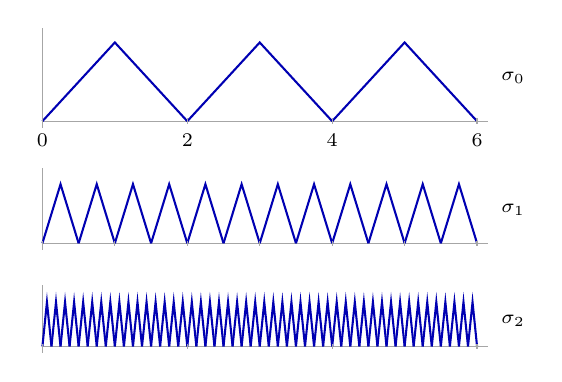
\begin{tikzpicture}[
  x=0.92cm,
  y=1.0cm,
  every node/.style={font=\scriptsize},
  axis/.style={gray!70, line width=0.45pt},
  wave/.style={blue!70!black, line width=0.75pt}
]
  % sigma_0 row
  \draw[axis] (0,0) -- (6.15,0);
  \draw[axis] (0,-0.08) -- (0,1.18);
  \foreach \i in {0,1,2} {
    \pgfmathsetmacro{\a}{2*\i}
    \pgfmathsetmacro{\b}{\a+1}
    \pgfmathsetmacro{\c}{\a+2}
    \draw[wave] (\a,0) -- (\b,1) -- (\c,0);
  }
  \foreach \x in {0,2,4,6} {
    \draw[axis] (\x,0.04) -- (\x,-0.04);
    \node[below] at (\x,-0.04) {$\x$};
  }
  \node[right] at (6.2,0.55) {$\sigma_0$};

  % sigma_1 row
  \begin{scope}[yshift=-1.55cm]
    \draw[axis] (0,0) -- (6.15,0);
    \draw[axis] (0,-0.08) -- (0,0.95);
    \foreach \i in {0,...,11} {
      \pgfmathsetmacro{\a}{0.5*\i}
      \pgfmathsetmacro{\b}{\a+0.25}
      \pgfmathsetmacro{\c}{\a+0.5}
      \draw[wave] (\a,0) -- (\b,0.75) -- (\c,0);
    }
    \foreach \x in {0,1,2,3,4,5,6} {
      \draw[axis] (\x,0.035) -- (\x,-0.035);
    }
    \node[right] at (6.2,0.42) {$\sigma_1$};
  \end{scope}

  % sigma_2 row
  \begin{scope}[yshift=-2.86cm]
    \draw[axis] (0,0) -- (6.15,0);
    \draw[axis] (0,-0.08) -- (0,0.78);
    \foreach \i in {0,...,47} {
      \pgfmathsetmacro{\a}{0.125*\i}
      \pgfmathsetmacro{\b}{\a+0.0625}
      \pgfmathsetmacro{\c}{\a+0.125}
      \draw[wave] (\a,0) -- (\b,0.5625) -- (\c,0);
    }
    \foreach \x in {0,2,4,6} {
      \draw[axis] (\x,0.03) -- (\x,-0.03);
    }
    \node[right] at (6.2,0.32) {$\sigma_2$};
  \end{scope}
\end{tikzpicture}

  \caption{The first compressed sawtooth terms $\sigma_k(x)=(3/4)^k\varphi(4^kx)$: heights shrink, slopes grow.}
  \label{fig:takagi-sawtooth-building-block}
\end{figure}

\begin{perspective} \label{per:nowhere-differentiability-explicit-and-generic} \hlt{Explicit Versus Generic Pathology}\\
The sawtooth series proves existence; Baire category shows nowhere differentiability is residual in $C([a,b],\R)$.
\end{perspective}

\begin{theorem} \label{thm:differentiable-somewhere-first-category} \hlt{Generic Nowhere Differentiability on Compact Intervals}\\
Let $a<b$, and let $C=C([a,b],\R)$ with the supremum metric. There exists a residual set $\mathcal{G}\subseteq C$ such that:
\begin{enumerate}[label=(\roman*)]
\setlength{\itemsep}{0pt}
\item no $f\in\mathcal{G}$ has an available one-sided derivative at any point of $[a,b]$;
\item no $f\in\mathcal{G}$ is monotone on any nondegenerate subinterval of $[a,b]$;
\item the set $\{f\in C:f\text{ is differentiable at some point of }[a,b]\}$ is first category.
\end{enumerate}
\begin{proof}
\begin{enumerate}[label=(\roman*)]
\setlength{\itemsep}{0pt}
\item Write $\Delta_hf(x)\defeq f(x+h)-f(x)$, and choose $N_0$ with $1/N_0<b-a$. For $n\geq N_0$, define
\begin{align}
R_n&\defeq\left\{f\in C:\forall x\in[a,b-1/n]\ \exists h>0\text{ with }\left|\frac{\Delta_hf(x)}{h}\right|>n\right\}, \nonumber\\
L_n&\defeq\left\{f\in C:\forall x\in[a+1/n,b]\ \exists h<0\text{ with }\left|\frac{\Delta_hf(x)}{h}\right|>n\right\}, \nonumber\\
G_n&\defeq\{f\in C:f\text{ is nonmonotone on every subinterval of length }1/n\}. \nonumber
\end{align}
Each $R_n,L_n,G_n$ is open and dense in $C$ (Weierstrass Approximation Theorem \ref{thm:weierstrass-polynomial-approximation}), plus small high-slope sawtooth perturbation; openness follows from compactness and uniform perturbation estimates.
\item Set $\mathcal{G}\defeq\bigcap_{n\geq N_0}(R_n\cap L_n\cap G_n)$. By Definition \ref{def:residual-thick-generic-set}, $\mathcal{G}$ is residual. If $f\in\mathcal{G}$, then the $R_n$ and $L_n$ conditions give one-sided difference quotients of arbitrarily large absolute value; since $f$ is bounded, the corresponding increments tend to $0$. Thus no available one-sided derivative exists.
\item Let $f\in\mathcal{G}$. Every nondegenerate subinterval contains a subinterval of length $1/n$ for all sufficiently large $n$, so the $G_n$ conditions make $f$ nonmonotone on every nondegenerate subinterval. If $f$ is differentiable somewhere, then $f\notin\mathcal{G}$; hence the differentiable-somewhere set lies in $C\setminus\mathcal{G}$, which is first category.
\end{enumerate}
\hlt{Structural Commentary}: Baire category turns dense sawtooth perturbability into a generic regularity failure.\\
\hlt{Key Insight}: The explicit construction shows existence; the category proof shows typicality.
\end{proof}
\end{theorem}

\begin{definition} \label{def:pointwise-uniform-bounded-equicontinuous} \hlt{Boundedness and Equicontinuity of Function Families}\\
Let $\mathcal{F}$ be a family of functions from $E$ into a metric space $(Y,d_Y)$; in scalar cases, take $d_Y(u,v)=\abs{u-v}$.
\begin{enumerate}[label=(\roman*)]
\setlength{\itemsep}{0pt}
\item $(f_n)$ is \hlt{pointwise bounded} on $E$ if $(f_n(x))$ is bounded in $Y$ for each $x\in E$.
\item A scalar sequence $(f_n)$ is \hlt{uniformly bounded} on $E$ if $\exists M$ such that $\abs{f_n(x)}<M$ for all $x\in E,n\in\N$.
\item If $E$ lies in a metric space $(X,d_X)$, then $\mathcal{F}$ is \hlt{equicontinuous} on $E$ if $\forall\varepsilon>0$ $\exists\delta>0$,\\
such that $d_X(x,y)<\delta,\ x,y\in E,\ f\in\mathcal{F}$ $\Longrightarrow$ $d_Y(f(x),f(y))<\varepsilon$.
\item The family is \hlt{pointwise equicontinuous} if for every $p\in E$ and $\varepsilon>0$ there is $\delta=\delta(p,\varepsilon)>0$ such that $d_X(p,y)<\delta,\ y\in E,\ f\in\mathcal{F}$ implies $d_Y(f(p),f(y))<\varepsilon$.
\end{enumerate}
\end{definition}

\begin{figure}[H]
  \centering
  \begin{tikzpicture}[
  >=Stealth,
  x=0.82cm,
  y=0.86cm,
  every node/.style={font=\scriptsize},
  axis/.style={->, gray!70, line width=0.55pt},
  curvea/.style={blue!70!black, line width=0.9pt},
  curveb/.style={orange!85!black, line width=0.9pt},
  curvec/.style={teal!70!black, line width=0.9pt},
  guide/.style={gray!55, dashed, line width=0.5pt},
  domainband/.style={teal!10},
  epsbar/.style={black!65, line width=0.8pt},
  point/.style={circle, fill=black, inner sep=1.15pt}
]
  \draw[axis] (-0.35,0) -- (7.25,0) node[right] {$x$};
  \draw[axis] (0,-0.25) -- (0,3.7) node[above] {$y$};

  \path[domainband] (2.65,0) rectangle (4.35,3.35);
  \draw[guide] (2.65,0) -- (2.65,3.35);
  \draw[guide] (3.5,0) -- (3.5,3.35);
  \draw[guide] (4.35,0) -- (4.35,3.35);
  \node[below] at (2.65,0) {$p-\delta$};
  \node[below] at (3.5,0) {$p$};
  \node[below] at (4.35,0) {$p+\delta$};

  \draw[curvea] plot[smooth, tension=0.75] coordinates {
    (0.65,2.73) (1.55,2.88) (2.65,2.90) (3.5,2.82)
    (4.35,2.68) (5.45,2.56) (6.55,2.58)
  };
  \draw[curveb] plot[smooth, tension=0.75] coordinates {
    (0.65,1.86) (1.70,1.82) (2.65,1.83) (3.5,1.87)
    (4.35,1.95) (5.45,2.12) (6.55,2.20)
  };
  \draw[curvec] plot[smooth, tension=0.75] coordinates {
    (0.65,1.42) (1.65,1.43) (2.65,1.30) (3.5,1.11)
    (4.35,1.00) (5.45,0.85) (6.55,0.82)
  };

  \foreach \y in {2.82,1.87,1.11} {
    \node[point] at (3.5,\y) {};
  }

  \foreach \x/\y in {2.78/2.82,4.22/2.82,2.78/1.87,4.22/1.87,2.78/1.11,4.22/1.11} {
    \draw[epsbar] (\x,\y-0.18) -- (\x,\y+0.18);
  }

  \node[above] at (1.15,2.96) {$\mathcal{F}$};
  \node[black!65, right] at (4.36,2.82) {$\varepsilon$};
\end{tikzpicture}

  \caption{One input scale $\delta$ controls every curve in $\mathcal F$ within tolerance $\varepsilon$.}
  \label{fig:equicontinuity-family-schematic}
\end{figure}

\begin{theorem} \label{thm:pointwise-equicontinuity-compact-uniform} \hlt{Pointwise Equicontinuity Becomes Uniform on Compact Sets}\\
Every pointwise equicontinuous family $\mathcal{F}\subset C(K,\C)$ on compact $K$ is equicontinuous.
\begin{proof}
Otherwise, choose $\varepsilon>0$, $f_n\in\mathcal{F}$, and $x_n,t_n\in K$ with $d(x_n,t_n)<1/n$ but $\abs{f_n(x_n)-f_n(t_n)}\geq\varepsilon$.\\
By Theorem \ref{thm:compact-sequential-subsequence}, pass to $x_n\to x_0$; then $t_n\to x_0$ too.\\
Pointwise equicontinuity at $x_0$ gives $\abs{f_n(x_n)-f_n(t_n)}<\varepsilon$ for large $n$, a contradiction.\\
\hlt{Structural Commentary}: Compactness turns moving counterexamples into one base point.\\
\hlt{Key Insight}: The local $\delta(x,\varepsilon)$ becomes one uniform $\delta$ only after compactness prevents escape.
\end{proof}
\end{theorem}

\begin{example} \label{ex:uniform-boundedness-without-uniform-subsequence} \hlt{Uniform Boundedness Alone Is Not Enough}\\
On $[0,1]$, let $f_n(x)\defeq \frac{x^2}{x^2+(1-nx)^2}$. Then $\abs{f_n}\leq1$ and $f_n\to0$ pointwise, but $f_n(1/n)=1$; hence no uniformly convergent subsequence. The missing hypothesis is equicontinuity.
\end{example}

\begin{theorem} \label{thm:diagonal-selection-countable-pointwise} \hlt{Diagonal Selection on a Countable Set}\\
Every pointwise bounded sequence $(f_n)$ on countable $E$ has a subsequence converging pointwise on $E$.
\begin{proof}
List $E=\{x_1,x_2,\ldots\}$. Inductively choose nested subsequences $S_i$ so that $S_i(x_i)$ converges.\\
The diagonal subsequence is eventually contained in each $S_i$, hence converges at every $x_i$.\\
\hlt{Structural Commentary}: The diagonal keeps the $i$th convergence property after the $i$th step.\\
\hlt{Key Insight}: Countability permits diagonal convergence.
\end{proof}
\end{theorem}

\begin{theorem} \label{thm:uniform-convergence-implies-equicontinuity-on-compact} \hlt{Uniform Convergence Implies Equicontinuity on Compact Sets}\\
If $K$ is compact, $f_n\in C_b(K)$, and $f_n\rightrightarrows f$ on $K$, then $\{f_n:n\in\N\}$ is equicontinuous.
\begin{proof}
Choose $N$ so $\norm{f_n-f_N}_{\infty}<\varepsilon$ for $n>N$.\\
By Theorem \ref{thm:compact-continuity-uniform-continuity}, choose one $\delta>0$ giving $\varepsilon$-control for $f_1,\ldots,f_N$.\\
If $n>N$, $d(x,y)<\delta$, then $\abs{f_n(x)-f_n(y)} \leq \abs{f_n(x)-f_N(x)}+\abs{f_N(x)-f_N(y)}+\abs{f_N(y)-f_n(y)}<3\varepsilon$.\\
Together with the finite initial family, $\{f_n\}$ is equicontinuous.\\
\hlt{Structural Commentary}: A uniformly convergent tail stays close to one uniformly continuous function.\\
\hlt{Key Insight}: Compactness handles finitely many functions; uniform convergence handles the tail.
\end{proof}
\end{theorem}

\begin{theorem} \label{thm:arzela-ascoli-compact-metric} \hlt{Arzela--Ascoli Selection Theorem}\\
Let $K$ be compact. If $(f_n)\subset C_b(K)$ is pointwise bounded and equicontinuous on $K$, then:
\begin{enumerate}[label=(\roman*)]
\setlength{\itemsep}{0pt}
\item $(f_n)$ is uniformly bounded on $K$;
\item $(f_n)$ contains a uniformly convergent subsequence.
\end{enumerate}
\begin{proof}
\begin{enumerate}[label=(\roman*)]
\setlength{\itemsep}{0pt}
\item Choose $\delta>0$ from equicontinuity with tolerance $1$. Compactness gives $K\subseteq\bigcup_{j=1}^{r}B_{\delta}(p_j)$.\\
Pointwise boundedness gives $M_j$ such that $\abs{f_n(p_j)}\leq M_j \forall n$.\\
If $x\in B_{\delta}(p_j)$, then $\abs{f_n(x)}\leq\abs{f_n(x)-f_n(p_j)}+\abs{f_n(p_j)}<1+M_j$, seq uniformly bounded by $1+\max_jM_j$.
\item For each $m$, compactness gives a finite $1/m$-net in $K$; the union of these finite nets is a countable dense set $E\subset K$. By Theorem \ref{thm:diagonal-selection-countable-pointwise}, some subsequence $(g_i)$ converges pointwise on $E$.\\
Given $\varepsilon>0$, choose $\delta>0$ from equicontinuity with tolerance $\varepsilon/3$, and points $x_1,\ldots,x_r\in E$ with $K\subseteq\bigcup_sB_{\delta}(x_s)$. As $(g_i(x_s))$ converges for each of finitely many $x_s$, $\exists N$ s.t. $i,j\geq N$ implies $\abs{g_i(x_s)-g_j(x_s)}<\varepsilon/3 \ \forall s$. If $d(x,x_s)<\delta$, then $\abs{g_i(x)-g_j(x)} \leq\abs{g_i(x)-g_i(x_s)}+\abs{g_i(x_s)-g_j(x_s)}+\abs{g_j(x_s)-g_j(x)} <\varepsilon$.\\
Thus $(g_i)$ is uniformly Cauchy and converges uniformly by Theorem \ref{thm:uniform-cauchy-criterion}.
\end{enumerate}
\hlt{Structural Commentary}: Dense convergence plus equicontinuity becomes uniform convergence.\\
\hlt{Key Insight}: Equicontinuity is exactly the compactness-compatible hypothesis missing from Example \ref{ex:uniform-boundedness-without-uniform-subsequence}.
\end{proof}
\end{theorem}

\begin{figure}[H]
  \centering
  \begin{tikzpicture}[
  >=Stealth,
  x=0.88cm,
  y=0.88cm,
  every node/.style={font=\scriptsize},
  cloud/.style={circle, fill=gray!32, inner sep=1.05pt},
  chosen/.style={circle, fill=orange!82!black, inner sep=1.45pt},
  limit/.style={circle, fill=blue!70!black, inner sep=1.9pt},
  arrow/.style={->, orange!82!black, line width=0.72pt},
  note/.style={fill=white, inner sep=0.8pt}
]
  \foreach \x/\y in {
    0.55/2.20,0.85/1.05,1.18/1.70,1.48/2.55,1.78/0.82,
    2.08/1.62,2.42/2.05,2.75/1.20,3.08/1.52,3.38/1.33,
    3.72/1.42,4.05/1.34,4.42/1.37
  } {
    \node[cloud] at (\x,\y) {};
  }

  \foreach \x/\y/\lab in {
    1.18/1.70/{f_{n_1}},
    2.08/1.62/{f_{n_2}},
    3.08/1.52/{f_{n_3}},
    4.05/1.34/{f_{n_4}}
  } {
    \node[chosen] at (\x,\y) {};
    \node[note, above=2pt] at (\x,\y) {$\lab$};
  }
  \node[limit] at (5.10,1.32) {};
  \node[note, right=2pt] at (5.10,1.32) {$f$};

  \draw[arrow] (1.29,1.69) -- (1.96,1.63);
  \draw[arrow] (2.19,1.61) -- (2.96,1.53);
  \draw[arrow] (3.19,1.50) -- (3.93,1.35);
  \draw[arrow] (4.17,1.34) -- (4.88,1.32);
\end{tikzpicture}

  \caption{Arzela--Ascoli selects a uniformly convergent subsequence.}
  \label{fig:sequential-compactness-subsequence}
\end{figure}

\begin{definition} \label{def:sigma-compact-metric-space} \hlt{$\sigma$-Compact Metric Space}\\
A metric space $X$ is \hlt{$\sigma$-compact} if $X=\bigcup\limits_{j=1}^{\infty}K_j$ for compact subsets $K_j\subseteq X$.
\end{definition}

\begin{theorem} \label{thm:arzela-ascoli-sigma-compact-locally-uniform} \hlt{Arzela--Ascoli on $\sigma$-Compact Spaces}\\
Let $X$ be $\sigma$-compact, $Y$ a metric space, and $(f_n)$ pointwise equicontinuous maps $X\to Y$. If each orbit $\{f_n(x):n\in\N\}$ lies in a compact subset of $Y$, then some subsequence converges uniformly on compact subsets of $X$.
\begin{proof}
Choose an increasing compact exhaustion $X=\bigcup_jK_j$.\\
By Theorem \ref{thm:pointwise-equicontinuity-compact-uniform}, each restriction $f_n|_{K_j}$ is uniformly equicontinuous. Applying Theorem \ref{thm:arzela-ascoli-compact-metric} on $K_1,K_2,\ldots$ and diagonalizing gives a subsequence $(g_m)$ converging uniformly on every $K_j$, hence pointwise on $X$.\\
If $K\subseteq X$ is compact, then $(g_m|_K)$ is uniformly equicontinuous, and a finite-net argument upgrades pointwise convergence on $K$ to uniform convergence on $K$.\\
\hlt{Structural Commentary}: Exhaust $X$ by compact pieces and diagonalize the compact theorem.\\
\hlt{Key Insight}: Local uniform convergence replaces global uniform convergence.
\end{proof}
\end{theorem}

\begin{corollary} \label{cor:arzela-ascoli-real-line-locally-uniform} \hlt{Real-Line Local Uniform Subsequence}\\
If $(f_n)$ is pointwise equicontinuous on $\R$ and bounded at one point, then it has a subsequence converging uniformly on compact subsets of $\R$.
\begin{proof}
Let $(f_n(x_0))$ be bounded. On any compact interval containing $x_0$, Theorem \ref{thm:pointwise-equicontinuity-compact-uniform} gives uniform equicontinuity; finitely many $\delta$-steps from $x_0$ to $x$ bound each orbit $(f_n(x))$. Hence Theorem \ref{thm:arzela-ascoli-sigma-compact-locally-uniform} applies on $\R$.
\hlt{Structural Commentary}: One bounded anchor propagates across compact intervals.\\
\hlt{Key Insight}: Pointwise equicontinuity turns local boundedness into compactwise compactness.
\end{proof}
\end{corollary}

\begin{method} \label{meth:function-space-compactness-proof-patterns} \hlt{Function-Space Compactness Proof Patterns}
\begin{enumerate}[label=(\roman*)]
\setlength{\itemsep}{0pt}
\item \hlt{Completeness}: prove a function sequence is uniformly Cauchy, build the pointwise limit, and use uniform convergence to keep continuity or boundedness.
\item \hlt{Baire category}: show a desired property contains a countable intersection of dense open subsets of a complete function space.
\item \hlt{Compactness/equicontinuity}: pass from finite nets to all of $K$.
\item \hlt{Diagonal selection}: get pointwise convergence on a countable dense set, then upgrade using equicontinuity.
\item \hlt{Locally uniform}: exhaust a $\sigma$-compact domain by compact sets and diagonalize.
\end{enumerate}
\hlt{Key Insight}: Compactness in function spaces is finite-net control plus equicontinuity.
\end{method}
